\chapter{Microbiotes et symbioses}\label{ch:b3:microbiomes}

Vous portez environ trente-huit mille milliards de bactéries, à peu
près une pour chacune de vos propres cellules, la plupart dans le
dernier mètre de votre intestin, où elles pèsent à peu près autant que
votre cerveau et portent cent fois plus de gènes que vous. Une souris
élevée sans aucune d'elles a besoin d'un tiers de nourriture en plus
pour tenir son poids, a un système immunitaire rabougri et se comporte
bizarrement. Un pois donne un dixième de son sucre à des bactéries
logées dans des nodules de ses racines et reçoit son azote en retour~;
quatre plantes terrestres sur cinq échangent du sucre contre du
phosphate avec des champignons enroulés autour de leurs racines, comme
elles le font depuis quatre cents millions d'années~; un corail est un
animal qui cultive des algues dans ses cellules et meurt quand la mer
se réchauffe assez pour qu'il les expulse. Les êtres vivants ne sont pas
des individus mais des consortiums, et ce chapitre traite de la
biologie de ces associations~: comment on les dénombre et les
caractérise par séquençage, ce que les partenaires échangent, comment
l'échange se négocie et se surveille, et pourquoi certains partenaires
finissent en organites.

\section{Des mots pour vivre ensemble}

\begin{definition}[La symbiose]\label{def:b3:microbiomes:symbiosis}
\index{symbiose}\index{mutualisme}\index{commensalisme}\index{holobionte}\index{microbiote}\index{transmission verticale}
La \emph{symbiose} est l'association durable et intime d'organismes
d'espèces différentes~; c'est un \emph{mutualisme} si les deux y
gagnent, un \emph{commensalisme} si l'un y gagne et que l'autre n'y
perd ni n'y gagne, et un parasitisme si l'un y gagne aux dépens de
l'autre --- et un même couple peut se déplacer le long de cette ligne
selon les circonstances. Un \emph{endosymbionte} vit à l'intérieur des
cellules de son hôte~; un partenaire \emph{obligatoire} ne peut pas
vivre seul. Les symbiontes sont transmis \emph{verticalement}, du
parent à sa descendance (les \emph{Buchnera} du puceron passent par
l'œuf), ou \emph{horizontalement}, acquis à neuf à chaque génération
depuis le milieu ou depuis d'autres hôtes (le \emph{Vibrio} du calmar,
les bactéries de l'intestin humain). Le \emph{microbiote} est la
communauté entière des microbes d'un habitat --- un intestin, la
surface d'une feuille, un gramme de sol --- et l'\emph{holobionte} est
un hôte avec son microbiote, considéré comme l'unité que voit la
sélection naturelle.
\end{definition}

\begin{example}[Trois partenaires obligatoires]\label{ex:b3:microbiomes:obligate}
Le \emph{Buchnera} du puceron vit dans les cellules de son hôte depuis
deux cents millions d'années, fabrique les acides aminés essentiels qui
manquent à la sève élaborée, et a réduit son génome à \qty{640}{kb} ---
le septième de celui de ses parents libres --- en perdant tous les
gènes que l'hôte fournit désormais. La bactérie \emph{Wolbachia},
présente chez deux tiers des espèces d'insectes, ne se transmet que par
les œufs, et a donc évolué à favoriser les femelles~: elle tue les
embryons mâles, les féminise, ou fait mourir les œufs de femelles non
infectées lorsqu'ils sont fécondés par des mâles infectés
(l'\emph{incompatibilité cytoplasmique}), ce qui la répand dans une
population~; les moustiques qui la portent transmettent mal la dengue,
et en lâcher a fait reculer la dengue dans plusieurs villes. L'amibe
\emph{Paulinella} a capté il y a une centaine de millions d'années une
cyanobactérie qui n'est aujourd'hui ni tout à fait une bactérie ni tout
à fait un chloroplaste --- une seconde origine, indépendante, des
organites photosynthétiques, saisie à mi-chemin.
\end{example}

\section{Dénombrer une communauté}

\begin{method}[Établir le profil d'un microbiote par séquençage]\label{met:b3:microbiomes:16s}
\index{séquençage de l'ARNr 16S}\index{métagénomique}\index{unité taxinomique opérationnelle}
La plupart des microbes ne se cultivent pas~; on les dénombre par leur
ADN. (1) Extraire l'ADN de l'échantillon --- fèces, sol, eau de mer
filtrée sur une membrane. (2) Ou bien amplifier le gène de l'ARN
ribosomique de la petite sous-unité (le \emph{16S}) avec des \omterm{def:b3:genetic-engineering:pcr}{amorces}
qui s'apparient à ses régions universelles, et séquencer les régions
variables entre elles --- une enquête par \emph{amplicon}, bon marché,
qui identifie les bactéries à peu près au genre et les dénombre par le
nombre de lectures~; ou bien séquencer tout l'ADN --- la
\emph{métagénomique shotgun}, qui récupère des gènes et des génomes
entiers et rend donc compte de ce que la communauté sait faire, et pas
seulement de qui s'y trouve. (3) Regrouper les lectures en variants de
séquence ou en \emph{\omterm{met:b3:microbiomes:16s}{unités taxinomiques opérationnelles}} (OTU,
conventionnellement à \qty{97}{\%} d'identité pour une «~espèce~»), les
assigner par comparaison avec des bases de données
(\cref{ch:b3:bioinformatics}), et dresser le tableau des comptes par
échantillon. (4) Calculer la diversité au sein d'un échantillon et
comparer les compositions entre échantillons. Les comptes sont
relatifs --- les lectures d'un échantillon font un total fixé --- et
sont biaisés par l'extraction, les \omterm{def:b3:genetic-engineering:pcr}{amorces} et le nombre de copies, de
sorte que les différences entre échantillons traités de la même façon
sont dignes de foi là où les nombres absolus ne le sont pas.
\end{method}

\begin{definition}[La diversité]\label{def:b3:microbiomes:diversity}
\index{richesse spécifique}\index{indice de Shannon}\index{indice de Simpson}\index{raréfaction}
Pour une communauté de $S$ espèces d'abondances relatives $p_{1},\dots,
p_{S}$ ($\sum p_{i} = 1$)~: la \emph{richesse} est $S$~; l'\emph{indice
de Shannon} $H = -\sum_{i} p_{i}\ln p_{i}$ mesure l'incertitude sur
l'espèce d'un individu tiré au hasard, et $e^{H}$ est le nombre
d'espèces également abondantes qui donnerait la même incertitude (le
nombre effectif d'espèces)~; l'\emph{indice de Simpson}
$D = \sum_{i} p_{i}^{2}$ est la probabilité que deux individus tirés au
hasard soient de la même espèce, et $1/D$ est un autre nombre effectif,
pondéré vers les espèces communes. La richesse dépend du nombre
d'individus examinés~: une \emph{courbe de raréfaction} porte les
espèces trouvées en fonction du nombre d'individus échantillonnés, et
s'aplatit quand la plupart des espèces ont été vues.
\end{definition}

\begin{theorem}[La raréfaction]\label{thm:b3:microbiomes:rarefaction}
\index{raréfaction!formule}\index{couverture de Good}
Un échantillon contient $N$ individus de $S$ espèces, dont $N_{i}$ de
l'espèce $i$. Le nombre espéré d'espèces dans un sous-échantillon
aléatoire de $n$ individus, tirés sans remise, vaut
\[
E[S_{n}] = \sum_{i=1}^{S}\left[1 - \frac{\binom{N - N_{i}}{n}}
{\binom{N}{n}}\right],
\]
qui croît avec $n$ et vaut $S$ en $n = N$. On compare deux échantillons
de tailles différentes en les raréfiant tous deux au même $n$. La
fraction des individus de la communauté qui appartiennent à des espèces
non encore vues s'estime par la \emph{\omterm{thm:b3:microbiomes:rarefaction}{couverture de Good}}~: environ
$f_{1}/N$, où $f_{1}$ est le nombre d'espèces vues exactement une fois
(les singletons).
\end{theorem}
\begin{proof}
L'espèce $i$ est absente du sous-échantillon exactement quand les $n$
individus sont tous tirés parmi les $N - N_{i}$ autres, ce qui arrive
dans $\binom{N - N_{i}}{n}$ des $\binom{N}{n}$ sous-échantillons
également probables~; l'espèce $i$ est donc présente avec la
probabilité $1 - \binom{N-N_{i}}{n}/
\binom{N}{n}$, et le nombre espéré d'espèces présentes est la somme de
ces probabilités (espérance d'une somme d'indicatrices). Chaque terme
croît avec $n$, et en $n = N$ tout binomial du numérateur est nul.
L'estimation de Good~: un individu tiré ensuite appartient à une espèce
non vue avec à peu près la probabilité qu'un individu de l'échantillon
pris au hasard ait été le seul de son espèce, $f_{1}/N$ (Good, 1953)~;
sa justification est admise ici.
\end{proof}

\begin{example}[Deux intestins]\label{ex:b3:microbiomes:two-guts}
Un échantillon de $1000$ lectures chez une personne donne $150$
espèces, avec $H = 3.5$ et $40$ singletons~; un échantillon de $5000$
lectures chez une autre en donne $260$. Le second n'est pas
nécessairement plus divers~: il a été échantillonné cinq fois plus
profondément, et le raréfier à $1000$ lectures peut donner $150$ aussi.
La couverture du premier échantillon vaut $1 - 40/1000 =
\qty{96}{\%}$~: quatre pour cent des bactéries de cet intestin
appartiennent à des espèces que l'échantillon n'a jamais vues, et un
échantillon plus profond les trouvera. Les nombres effectifs,
$e^{3.5} \approx 33$ espèces d'équitabilité contre une richesse de
$150$, disent que quelques espèces dominent --- ce à quoi ressemble
tout intestin.
\end{example}

\begin{omfigure}
\begin{tikzpicture}
\begin{axis}[
  width=0.68\linewidth, height=5.6cm,
  axis x line=bottom, axis y line=left,
  xmin=0, xmax=5000, ymin=0, ymax=300,
  xlabel={lectures échantillonnées, $n$}, ylabel={espèces observées},
  xlabel style={font=\small, at={(axis description cs:0.5,-0.12)}, anchor=north}, ylabel style={font=\small},
  tick label style={font=\small}, xtick={0,1000,2000,3000,4000,5000}, ytick={0,100,150,200,260},
  clip=false,
]
\addplot[very thick, omDef, domain=0:5000, samples=60] {260*(1-exp(-x/1500))};
\addplot[very thick, omThm, domain=0:1000, samples=30] {150*(1-exp(-x/300))*1.0};
\addplot[very thick, omThm, dashed, domain=1000:5000, samples=30] {150*(1-exp(-x/300))*1.0 + 8*(1-exp(-(x-1000)/2000))};
\draw[dashed, gray] (axis cs:1000,0) -- (axis cs:1000,300);
\node[font=\scriptsize, omDef, anchor=north west] at (axis cs:1200,292) {second intestin~: $260$ espèces à $5000$ lectures};
\node[font=\scriptsize, omThm, anchor=north east] at (axis cs:4900,140) {premier intestin~: $150$ à $1000$, près de son plateau};
\node[font=\scriptsize, gray, anchor=south west] at (axis cs:1050,10) {raréfier ici pour comparer};
\end{axis}
\end{tikzpicture}

{\small Courbes de \omterm{def:b3:microbiomes:diversity}{raréfaction}. Les espèces trouvées croissent avec les
lectures échantillonnées et s'aplatissent à mesure que la communauté
s'épuise~; on compare deux échantillons à la même profondeur. Ici le
second intestin monte encore à $5000$ lectures, de sorte que sa
richesse vraie est plus élevée encore.}
\end{omfigure}

\section{Le microbiote humain}

\begin{definition}[La communauté intestinale]\label{def:b3:microbiomes:gut}
\index{microbiote intestinal}\index{acide gras à chaîne courte}\index{résistance à la colonisation}\index{dysbiose}
L'intestin humain abrite environ $4\times 10^{13}$ bactéries, presque
toutes dans le côlon à $10^{11}$ par gramme de contenu, contre $10^{3}$
par gramme dans l'estomac acide et $10^{4}$--$10^{7}$ le long de
l'intestin grêle, dont le flux est rapide et la bile hostile. Cinq
cents à mille espèces par personne, la plupart de deux
embranchements, les Bacteroidetes et les Firmicutes, presque toutes
anaérobies~; le jeu de chaque personne est particulier et stable
pendant des années, fixé pour l'essentiel durant les trois premières
années de vie, à partir de la mère et du foyer. Ce qu'elles font~:
fermenter en \emph{acides gras à chaîne courte} --- acétate,
propionate, butyrate --- les fibres que les enzymes humaines ne savent
pas digérer, ce qui nourrit les cellules mêmes du côlon et fournit
jusqu'au dixième des calories de l'hôte~; fabriquer la vitamine~K et
quelques vitamines B~; transformer les acides biliaires et les
médicaments~; occuper chaque niche de sorte qu'un envahisseur ne trouve
aucune prise (la \emph{résistance à la colonisation})~; et éduquer le
système immunitaire, dont les lymphocytes~T régulateurs et les cellules
sécrétrices d'IgA se développent en réponse à elles
(\cref{ch:b3:adaptive-immunity}). Une communauté écartée de cet état
--- moins d'espèces, moins de fermenteurs, plus d'aérobies facultatifs
--- est une \emph{dysbiose}, observée dans les maladies inflammatoires
de l'intestin, après des \omterm{def:b3:bacteriology:antibiotics}{antibiotiques} et dans l'obésité, même si l'on
ne sait en général pas qui est la cause et qui l'effet.
\end{definition}

\begin{proof}[Faits expérimentaux]
Les souris élevées sans germes en isolateurs stériles (Gordon et ses
collègues, années 2000) ont des parois intestinales minces, de petits
organes lymphoïdes, peu d'anticorps, et ont besoin de \qty{30}{\%} de
calories en plus pour tenir leur poids~; colonisées par un \omterm{def:b3:microbiomes:symbiosis}{microbiote}
de souris normale, elles prennent du gras en deux semaines. Recevant le
\omterm{def:b3:microbiomes:symbiosis}{microbiote} d'une souris obèse plutôt que d'une souris maigre, des
souris sans germes ont pris plus de gras à nourriture égale
(Turnbaugh, 2006)~: la communauté elle-même modifie la récolte
d'énergie. Chez l'homme, la colite récidivante à
\emph{Clostridioides difficile} --- une \omterm{def:b3:microbiomes:gut}{dysbiose} où des \omterm{def:b3:bacteriology:antibiotics}{antibiotiques}
ont éliminé les concurrentes d'une sporulée productrice de toxine ---
a été guérie chez \qty{94}{\%} des patients par la perfusion des fèces
d'un donneur sain, contre \qty{31}{\%} avec l'\omterm{def:b3:bacteriology:antibiotics}{antibiotique} de référence
(van~Nood, 2013), premier essai randomisé où le médicament était une
communauté et non une molécule.
\end{proof}

\begin{omfigure}
\begin{tikzpicture}
\begin{axis}[
  width=0.68\linewidth, height=5.4cm,
  ybar, bar width=18pt,
  axis x line=bottom, axis y line=left,
  ymode=log, ymin=1, ymax=1e13,
  symbolic x coords={estomac, duodenum, jejunum, ileon, colon},
  xtick=data, xticklabels={estomac, duodénum, jéjunum, iléon, côlon},
  ytick={1e1,1e3,1e5,1e7,1e9,1e11},
  ylabel={bactéries par gramme de contenu},
  ylabel style={font=\small}, tick label style={font=\small},
  clip=false,
]
\addplot[fill=omDef!40, draw=omDef] coordinates {(estomac,1e3) (duodenum,1e4) (jejunum,1e5) (ileon,1e7) (colon,1e11)};
\node[font=\scriptsize, anchor=west, xshift=10pt] at (axis cs:estomac,3e3) {acide, pH 2};
\node[font=\scriptsize, anchor=south] at (axis cs:jejunum,1.5e5) {bile, flux rapide};
\node[font=\scriptsize, anchor=south, align=center] at (axis cs:colon,1.5e11) {lent, anaérobie~:\\le fermenteur};
\end{axis}
\end{tikzpicture}

{\small Densité bactérienne le long de l'intestin humain, en échelle
logarithmique~: une multiplication par cent millions de l'estomac acide
au côlon, où vivent presque tous les microbes du corps.}
\end{omfigure}

\begin{omfigure}
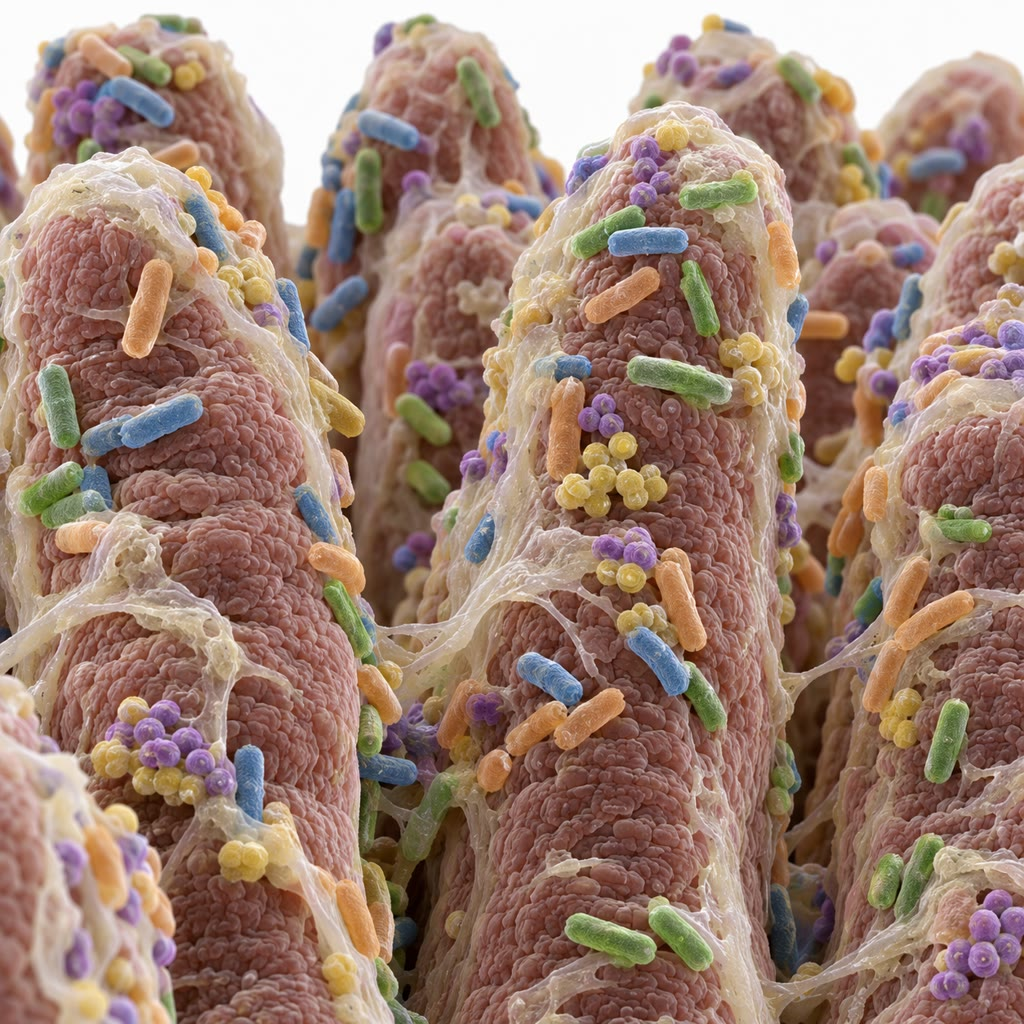
\includegraphics[width=0.40\linewidth]{images/book5/ai/b5-14-gut-microbiota.jpg}

{\small La surface de la paroi intestinale au microscope électronique à
balayage, des bactéries de plusieurs sortes logées dans le mucus entre
les villosités.}
\end{omfigure}

\section{Les plantes et leurs partenaires}

\begin{definition}[La symbiose légumineuse--rhizobium]\label{def:b3:microbiomes:nodule}
\index{rhizobiums}\index{nodule racinaire}\index{facteur Nod}\index{leghémoglobine}\index{nitrogénase}
Les légumineuses logent des bactéries fixatrices d'azote (les
\emph{rhizobiums}) dans des \emph{nodules racinaires}, organes bâtis
pour cela après un dialogue moléculaire. La racine sécrète des
flavonoïdes~; un rhizobium de l'espèce accordée répond par des
\emph{facteurs Nod} --- des lipochito-oligosaccharides dont les
décorations désignent le partenaire~; un récepteur kinase du poil
absorbant les fixe et déclenche des oscillations du calcium dans le
noyau, l'enroulement du poil autour des bactéries et un \emph{cordon
d'infection} qui progresse vers l'intérieur au travers des cellules
tandis que le cortex, plus bas, se met à se diviser en nodule. Les
bactéries sont libérées dans les cellules du nodule à l'intérieur de
membranes et se différencient en \emph{bactéroïdes} qui expriment la
\emph{nitrogénase}, l'enzyme qui réduit N$_{2}$ en ammoniac au prix de
seize ATP par molécule. La nitrogénase est détruite par le dioxygène,
et pourtant les bactéroïdes respirent fort~; le nodule résout la
contradiction par une barrière de diffusion et par la
\emph{leghémoglobine}, une hémoglobine végétale qui fixe fortement le
dioxygène et le convoie aux bactéroïdes à faible concentration libre
--- c'est elle qui rend rose un nodule coupé. La plante paie six à dix
pour cent de ses photosynthétats et reçoit l'essentiel de son azote~;
l'azote fixé par les cultures de légumineuses du monde approche celui
de l'industrie des engrais.
\end{definition}

\begin{omfigure}
\begin{tikzpicture}[every node/.style={font=\scriptsize}, >=stealth]
  % stage 1: root hair and bacteria, flavonoid / Nod factor exchange
  \begin{scope}
    \draw[thick, omMeth!60!black, fill=omMeth!15] (0,0) rectangle (1.2,3.0);
    \draw[thick, omMeth!60!black, fill=omMeth!15] (1.2,1.6) .. controls (2.4,1.7) and (2.6,2.6) .. (2.9,2.4) .. controls (2.5,2.3) and (2.3,1.4) .. (1.2,1.2) -- cycle;
    \foreach \p in {(3.1,2.7),(3.4,2.3),(3.3,1.9)} \fill[omProp] \p ellipse (0.14 and 0.07);
    \draw[->, omMeth!60!black, thick] (2.6,1.5) -- (3.2,1.4); \node[below, omMeth!60!black] at (3.0,1.35) {flavonoïdes};
    \draw[<-, omProp, thick] (2.5,2.85) -- (3.0,3.0); \node[above, omProp] at (2.4,2.95) {facteurs Nod};
    \node[below, align=center] at (1.6,-0.2) {1. dialogue~: poil absorbant\\et rhizobiums};
  \end{scope}
  % stage 2: curled hair, infection thread
  \begin{scope}[xshift=4.6cm]
    \draw[thick, omMeth!60!black, fill=omMeth!15] (0,0) rectangle (1.2,3.0);
    \draw[thick, omMeth!60!black, fill=omMeth!15] (1.2,1.6) .. controls (2.3,1.8) and (2.8,2.6) .. (2.2,2.8) .. controls (1.9,2.9) and (1.8,2.5) .. (2.0,2.4) .. controls (2.3,2.2) and (1.9,1.3) .. (1.2,1.2) -- cycle;
    \draw[omProp, very thick] (2.05,2.55) .. controls (1.8,2.1) and (1.4,1.7) .. (0.4,1.3);
    \foreach \p in {(1.85,2.3),(1.5,1.9),(1.1,1.6),(0.7,1.4)} \fill[omProp] \p ellipse (0.1 and 0.05);
    \node[right, omProp, font=\tiny] at (2.3,1.0) {cordon d'infection};
    \foreach \p in {(0.3,0.5),(0.6,0.7),(0.9,0.5)} \draw[omMeth!60!black] \p circle (0.12);
    \node[below, align=center] at (1.6,-0.2) {2. le poil s'enroule~; le cordon entre~;\\les cellules du cortex se divisent};
  \end{scope}
  % stage 3: nodule
  \begin{scope}[xshift=9.0cm]
    \draw[thick, omMeth!60!black, fill=omMeth!15] (0,0) rectangle (1.2,3.0);
    \draw[thick, omThm!60!black, fill=omThm!25] (1.2,1.5) ellipse (1.3 and 1.0);
    \foreach \p in {(1.0,1.5),(1.5,1.8),(1.6,1.2),(1.1,1.9),(1.2,1.1),(2.0,1.5)} \fill[omProp] \p circle (0.1);
    \node[right, align=left] at (2.6,2.0) {nodule~: bactéroïdes\\à nitrogénase};
    \node[right, align=left, omThm!60!black] at (2.6,1.1) {rose~: la leghémoglobine\\maintient O$_2$ bas};
    \draw[->, thick] (0.6,2.4) -- (1.0,2.0) node[pos=0, above] {sucre};
    \draw[<-, thick] (0.6,0.6) -- (1.0,1.0) node[pos=0, below] {NH$_3$};
    \node[below, align=center] at (1.6,-0.2) {3. les bactéroïdes fixent N$_2$~;\\du sucre contre de l'ammoniac};
  \end{scope}
\end{tikzpicture}

{\small Faire un nodule. Les flavonoïdes de la racine et les \omterm{def:b3:microbiomes:nodule}{facteurs
Nod} du rhizobium identifient les partenaires~; le poil absorbant
s'enroule, un cordon d'infection porte les bactéries vers l'intérieur,
et le cortex bâtit un nodule où des bactéroïdes, maintenus à faible
dioxygène par la \omterm{def:b3:microbiomes:nodule}{leghémoglobine}, fixent l'azote contre du sucre.}
\end{omfigure}

\begin{definition}[Les mycorhizes]\label{def:b3:microbiomes:mycorrhiza}
\index{mycorhize}\index{mycorhize arbusculaire}\index{voie commune de symbiose}
Les \emph{mycorhizes} sont des associations de racines et de
champignons, présentes chez quelque \qty{80}{\%} des espèces végétales
et dans les plus anciens fossiles de plantes terrestres. Dans les
\emph{mycorhizes arbusculaires} le champignon (un Gloméromycète) entre
dans les cellules de la racine et se ramifie en un arbuscule en forme
d'arbre au travers duquel phosphate, azote et eau passent à la plante
et sucres et lipides au champignon~; les hyphes du champignon
multiplient par cent la surface absorbante de la racine et atteignent
un phosphate que la racine n'atteint pas. Dans les
\emph{ectomycorhizes}, celles des arbres forestiers, le champignon
gaine la racine et croît entre les cellules. Les gènes végétaux qui
laissent entrer le champignon sont ceux de la même \emph{voie commune
de \omterm{def:b3:microbiomes:symbiosis}{symbiose}} --- récepteur, oscillations du calcium, facteurs de
transcription --- que les légumineuses réemploient pour les
\omterm{def:b3:microbiomes:nodule}{rhizobiums}~: le nodule est une invention tardive bâtie sur un
partenariat fongique de quatre cents millions d'années son aîné.
\end{definition}

\begin{proposition}[L'échange et sa surveillance]\label{prop:b3:microbiomes:sanctions}
\index{choix du partenaire}\index{sanctions}\index{tricheur}
Un \omterm{def:b3:microbiomes:symbiosis}{mutualisme} est un échange, et chaque partenaire est sélectionné pour
donner moins et prendre plus~; il tient parce que l'autre partenaire
peut riposter. Les légumineuses restreignent le dioxygène des nodules
dont les \omterm{def:b3:microbiomes:nodule}{rhizobiums} ne fixent rien, ce qui divise par deux leur
reproduction (Kiers, 2003)~: ce sont des \emph{sanctions}. Les plantes
d'un réseau mycorhizien allouent plus de carbone aux partenaires
fongiques qui livrent plus de phosphate, et les champignons plus de
phosphate aux racines qui paient plus de carbone --- un marché où
chacun récompense le meilleur négociant (Kiers, 2011). Les calmars
expulsent les bactéries de l'organe lumineux qui ne brillent pas~; le
système immunitaire humain tolère les commensaux qui restent dans la
lumière et attaque ceux qui franchissent la paroi. Là où un hôte ne
peut ni choisir ni sanctionner --- un endosymbionte hérité par l'œuf
--- l'\omterm{def:b3:bioinformatics:alignment}{alignement} des intérêts vient plutôt d'un destin commun~: un
symbionte à \omterm{def:b3:microbiomes:symbiosis}{transmission verticale} ne se reproduit que lorsque son hôte
se reproduit, et la sélection sur le symbionte favorise la reproduction
de l'hôte. Le mode de transmission prédit donc le caractère de
l'association~: la \omterm{def:b3:microbiomes:symbiosis}{transmission verticale} vers le \omterm{def:b3:microbiomes:symbiosis}{mutualisme} et la
dépendance, la transmission horizontale vers l'exploitation tenue en
bride par la surveillance.
\end{proposition}
\admitted

\begin{omfigure}
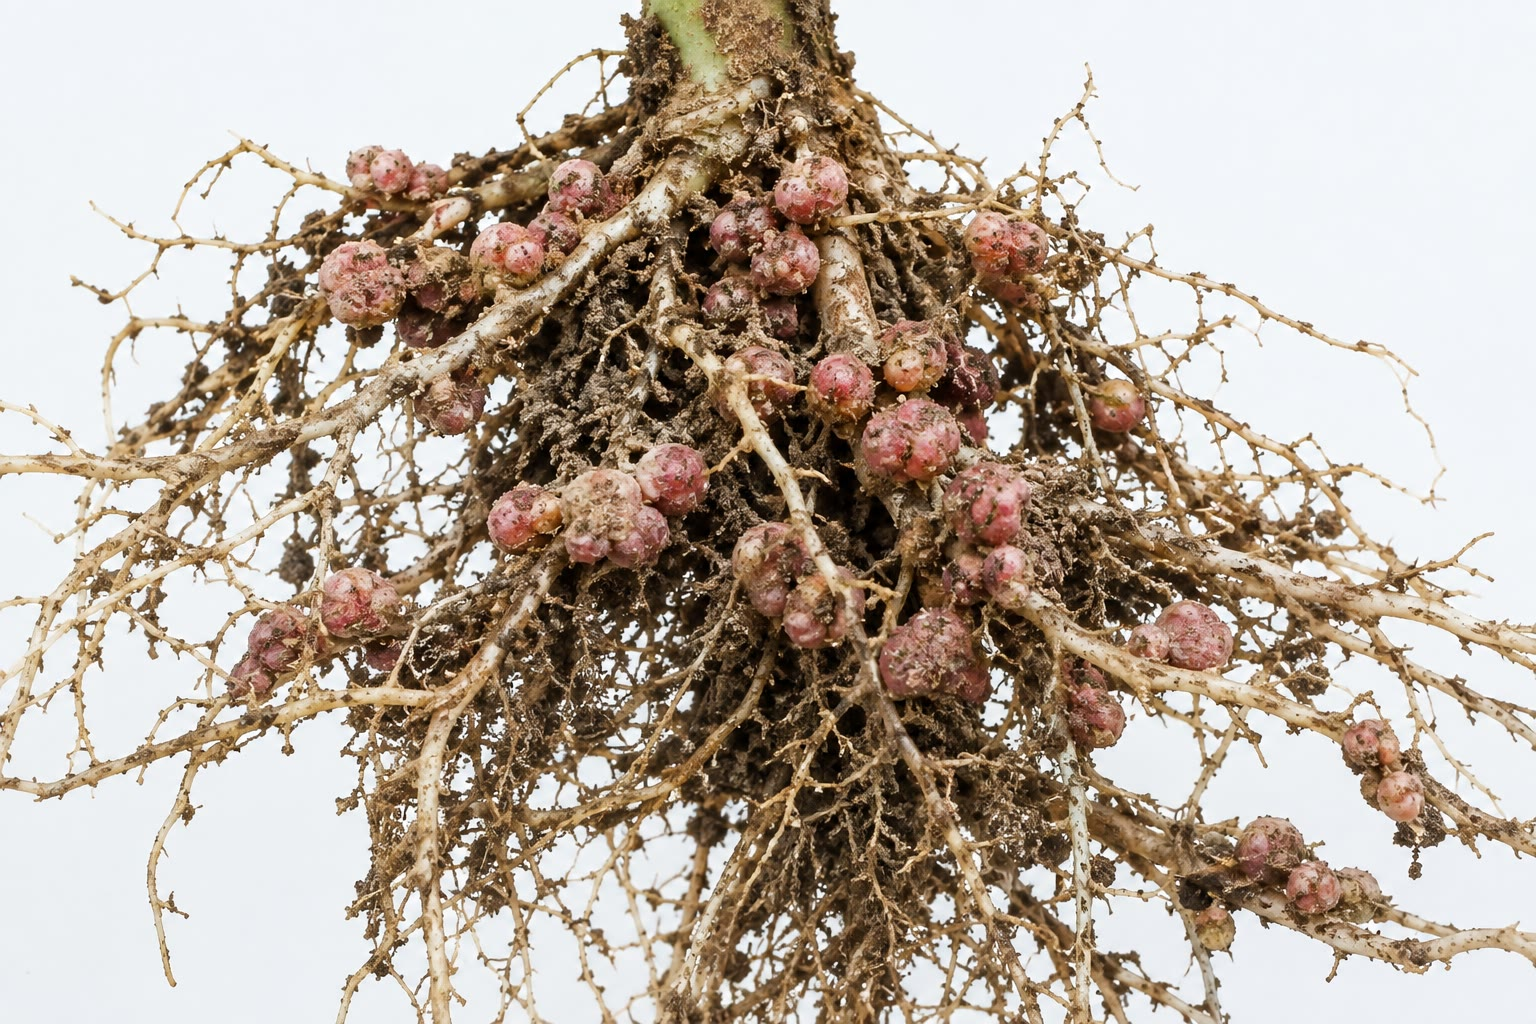
\includegraphics[width=0.46\linewidth]{images/book5/ai/b5-14-root-nodules.jpg}\hspace{0.04\linewidth}
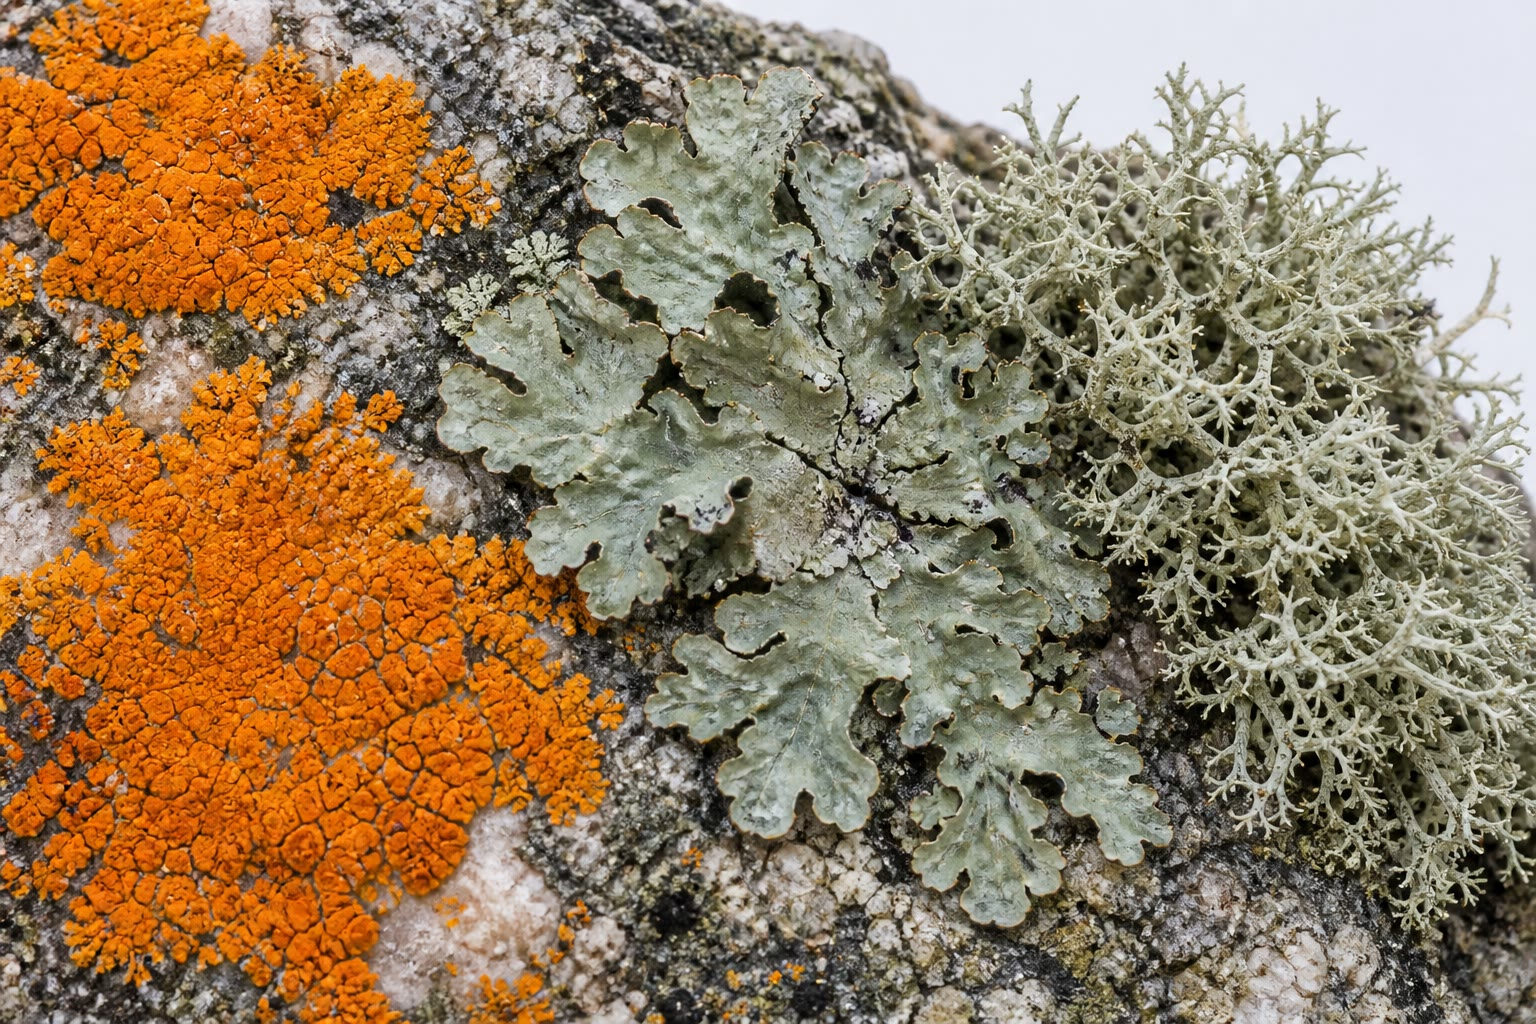
\includegraphics[width=0.46\linewidth]{images/book5/ai/b5-14-lichen.jpg}

{\small À gauche~: les racines nodulées d'une légumineuse, chaque nodule
rose étant une usine à azote de bactéroïdes nourris de sucre. À
droite~: des lichens sur la roche --- chacun un champignon qui loge une
algue ou une cyanobactérie photosynthétique, et qui ensemble colonisent
une surface qu'aucun des deux ne tiendrait seul.}
\end{omfigure}

\section{Des associations en mer et ailleurs}

\begin{definition}[Le corail et l'algue]\label{def:b3:microbiomes:coral}
\index{symbiose corallienne}\index{zooxanthelles}\index{blanchissement des coraux}
Les coraux bâtisseurs de récifs logent des algues dinoflagellées (les
\emph{Symbiodiniaceae}, les \emph{zooxanthelles}) dans les cellules de
leur paroi digestive, un million ou plus par centimètre carré. Les
algues font la photosynthèse dans le tissu de l'animal, en employant le
CO$_{2}$, l'ammoniac et le phosphate qu'il rejette, et lui rendent
jusqu'à \qty{90}{\%} du carbone qu'elles fixent sous forme de glycérol,
de sucres et d'acides aminés, qui nourrissent le corail et la
calcification qui bâtit le récif~; le corail, en retour, règle l'apport
d'azote des algues et donc leur croissance. L'association ne fonctionne
que dans une étroite fenêtre thermique~: quand l'eau reste un à deux
degrés au-dessus du maximum estival pendant quelques semaines, la
photosynthèse des algues est abîmée, elles libèrent de l'oxygène
réactif dans les cellules de l'hôte, et le corail les expulse --- c'est
le \emph{blanchissement}, le squelette blanc apparaissant au travers de
l'animal translucide. Un corail blanchi meurt de faim~; il se rétablit
si l'eau se refroidit en quelques semaines et meurt sinon. La fréquence
des blanchissements a quintuplé depuis 1980, et c'est par là que le
réchauffement efface les récifs.
\end{definition}

\begin{example}[Des symbioses qui font des habitats]\label{ex:b3:microbiomes:habitats}
Un \emph{lichen} est un champignon qui loge une algue verte ou une
cyanobactérie, le champignon fournissant la structure, la rétention
d'eau et les minéraux dissous de la roche, le photobionte fournissant
le sucre (et, si c'est une cyanobactérie, l'azote)~; les lichens
couvrent environ \qty{8}{\%} de la surface des terres, colonisent la
roche nue et amorcent sa conversion en sol. Le ver tubicole
\emph{Riftia} des sources hydrothermales n'a, adulte, ni bouche ni
intestin~; il loge des bactéries oxydant les sulfures dans un
trophosome et leur livre sulfure et dioxygène par une hémoglobine qui
fixe les deux, croissant de plus d'un mètre par an dans le noir sur de
l'énergie chimique. Les termites digèrent le bois grâce à une
communauté intestinale de protistes et de bactéries, et les ruminants
digèrent l'herbe grâce à un rumen de la taille d'une baignoire où
bactéries, archées et champignons fermentent la cellulose en acides
gras et en méthane~; la vache vit des acides gras et du corps même des
microbes. Dans chaque cas une capacité métabolique --- photosynthèse,
fixation de l'azote, oxydation des sulfures, digestion de la cellulose
--- que la lignée de l'hôte n'a jamais acquise par évolution a été
obtenue d'un coup par association.
\end{example}

\begin{omfigure}
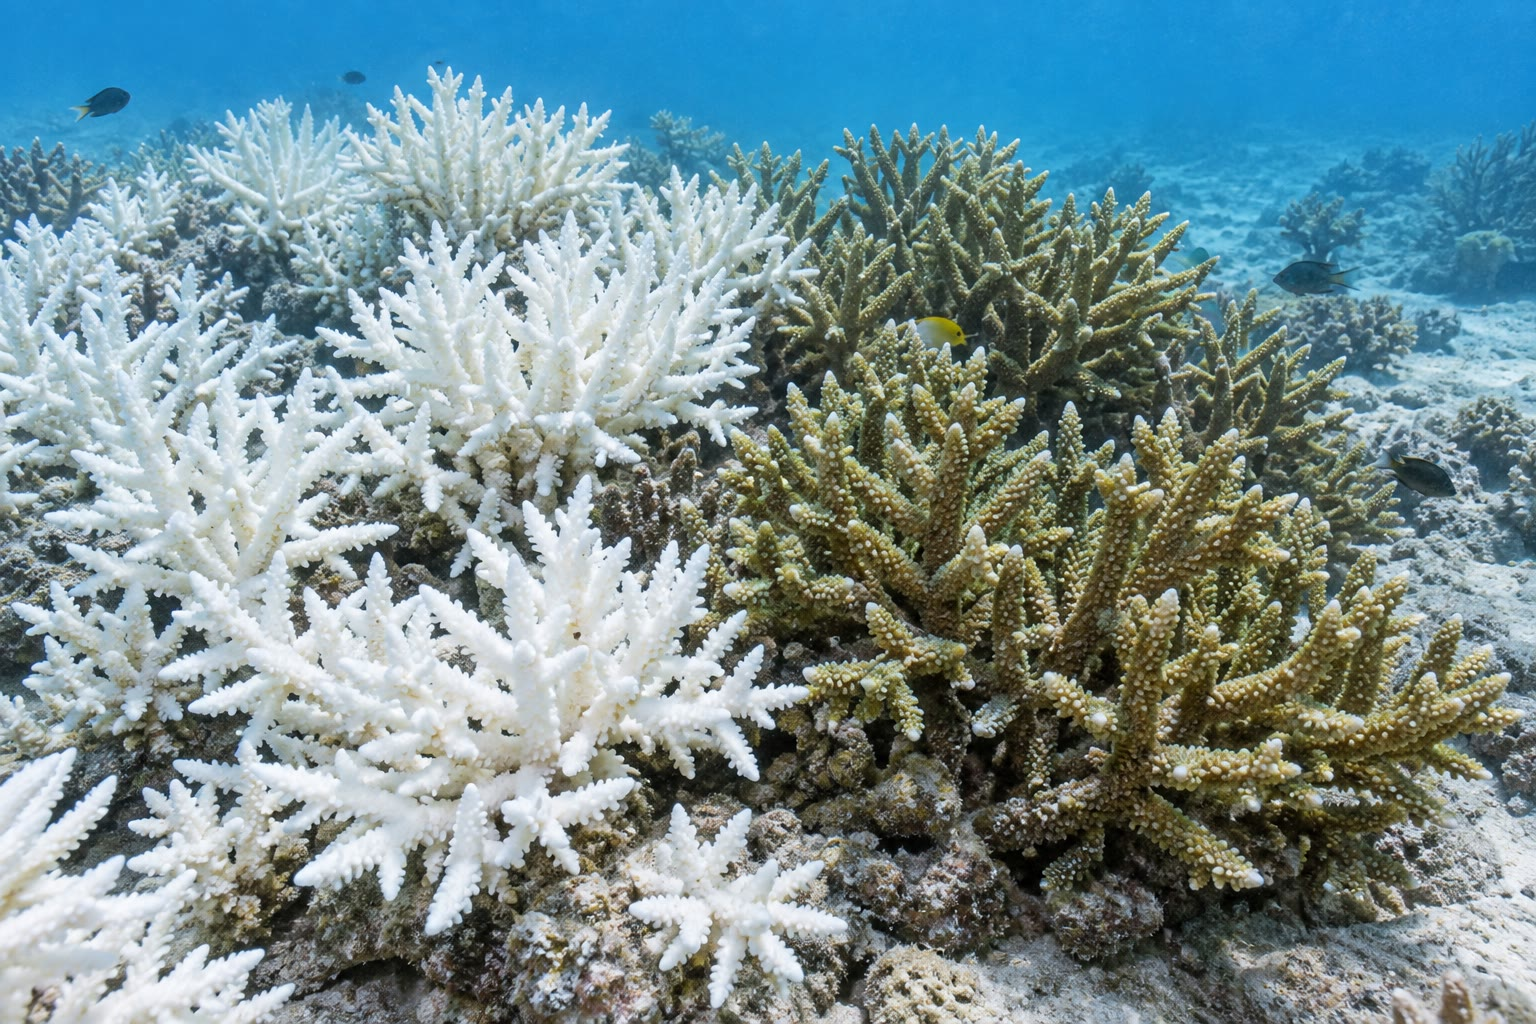
\includegraphics[width=0.56\linewidth]{images/book5/ai/b5-14-coral-bleaching.jpg}

{\small Un récif à demi blanchi~: les colonies blanches ont expulsé
leurs algues après des semaines d'eau trop chaude~; les brunes gardent
encore les leurs. Le corail blanc est vivant et affamé, et il a
quelques semaines pour être recolonisé.}
\end{omfigure}

\begin{omfigure}
\begin{tikzpicture}[every node/.style={font=\scriptsize}, >=stealth]
  % coral cell with alga
  \draw[very thick, omDef, fill=omDef!8] (0,0) ellipse (3.2 and 2.0); \node[above] at (0,2.05) {cellule de corail (gastroderme)};
  \draw[thick, omMeth!70!black, fill=omMeth!30] (-0.4,-0.1) circle (1.05); \node[align=center] at (-0.4,-0.1) {algue\\(zooxanthelle)};
  % exchanges
  \draw[->, thick, omMeth!70!black] (0.5,0.4) -- (1.9,0.9) node[right, align=left] {glycérol, sucres, acides aminés~:\\jusqu'à \qty{90}{\%} du carbone fixé};
  \draw[<-, thick, omThm] (0.5,-0.5) -- (1.9,-1.0) node[right, align=left] {CO$_2$, NH$_3$, phosphate\\(les déchets de l'animal)};
  \draw[<-, thick, omProp] (-1.3,0.3) -- (-2.6,1.0) node[left, align=right] {lumière au travers\\du tissu};
  \node[below, align=center] at (1.5,-2.1) {stress~: eau chaude des semaines $\to$ photosynthèse abîmée,\\oxygène réactif $\to$ algue expulsée $\to$ blanchissement};
  % thermometer-like bar on the right
  \begin{scope}[xshift=7.6cm, yshift=-1.6cm]
    \draw[thick] (0,0) rectangle (0.5,3.2);
    \fill[omDef!40] (0,0) rectangle (0.5,2.0); \fill[omProp!60] (0,2.0) rectangle (0.5,2.6); \fill[omThm!60] (0,2.6) rectangle (0.5,3.2);
    \node[right] at (0.6,1.0) {plage normale}; \node[right] at (0.6,2.3) {$+\qty{1}{\celsius}$~: stress}; \node[right, align=left] at (0.6,2.9) {$+\qty{2}{\celsius}$ des semaines~:\\blanchissement};
    \node[below, align=center] at (0.25,-0.1) {température estivale\\de la mer};
  \end{scope}
\end{tikzpicture}

{\small L'échange corail--algue~: l'algue fixe du carbone avec les
déchets de l'animal et la lumière qui traverse son tissu, et en rend
l'essentiel sous forme d'aliment~; une hausse petite mais soutenue de
la température rompt l'association.}
\end{omfigure}

\section{Du partenaire à l'organite}

\begin{proposition}[Réduction du génome et route vers l'organite]\label{prop:b3:microbiomes:reduction}
\index{réduction du génome}\index{transfert de gènes endosymbiotique}
Un endosymbionte hérité par l'œuf vit dans une population de quelques
cellules qui ne recombinent jamais avec l'extérieur. La sélection y est
faible (\cref{ch:b3:molecular-evolution}~: une petite population fixe
par dérive des mutations légèrement nuisibles), les gènes dont l'hôte
fournit les produits ne manquent à personne quand ils se cassent, et un
gène perdu ne se regagne jamais. Le génome rétrécit donc, génération
après génération --- \emph{Buchnera} jusqu'à \qty{640}{kb}, certains
symbiontes d'insectes jusqu'à \qty{140}{kb} et quelques centaines de
gènes, la mitochondrie jusqu'à \qty{16}{kb} et treize protéines chez
l'homme --- et le noyau de l'hôte acquiert des copies des gènes du
symbionte par \emph{\omterm{prop:b3:microbiomes:reduction}{transfert de gènes endosymbiotique}}, dont les
produits sont réimportés grâce à une séquence d'adressage. Quand l'hôte
fabrique la plupart des protéines du symbionte, commande sa division et
ne peut plus vivre sans lui, le symbionte est devenu un organite. Les
mitochondries et les plastes ont suivi cette route il y a deux
milliards et un milliard d'années (le volume de première année)~; le
chromatophore de \emph{Paulinella} est un troisième voyageur, cent
millions d'années plus loin.
\end{proposition}

\begin{remark}[L'individu revisité]\label{rem:b3:microbiomes:individual}
Un animal ou une plante est une communauté avec un génome en son
centre, dont l'essentiel du répertoire métabolique, et une bonne part
du développement et de l'immunité, dépend de partenaires qu'il n'a pas
hérités dans son propre ADN. Les conséquences pratiques sont déjà là~:
le \omterm{def:b3:microbiomes:symbiosis}{microbiote} comme médicament (la transplantation fécale), comme cible
de médicaments (les dégâts collatéraux des \omterm{def:b3:bacteriology:antibiotics}{antibiotiques}, les fibres
alimentaires en ordonnance), comme outil de diagnostic, et comme
moyen --- par des symbiontes modifiés et des moustiques porteurs de
\emph{Wolbachia} --- de changer la biologie de populations sauvages. La
conséquence théorique est que la sélection naturelle agit sur des
associations, et que les plus solides sont celles où le destin de l'un
est celui de l'autre.
\end{remark}

\section{Exercices}

\begin{exercise}[$\star$]\label{exo:b3:microbiomes:1}
Définir \omterm{def:b3:microbiomes:symbiosis}{mutualisme}, \omterm{def:b3:microbiomes:symbiosis}{commensalisme} et parasitisme, et donner un exemple
de chacun tiré de ce chapitre. Pourquoi un même couple d'espèces
peut-il passer d'une catégorie à l'autre~?
\end{exercise}

\begin{exercise}[$\star$]\label{exo:b3:microbiomes:2}
Calculer $H$, $e^{H}$, $D$ et $1/D$ pour une communauté d'abondances
$0.5$, $0.3$, $0.1$, $0.05$, $0.05$.
\end{exercise}

\begin{exercise}[$\star$]\label{exo:b3:microbiomes:3}
Opposer une enquête par amplicon 16S et une métagénomique shotgun~: que
rapporte chacune, et que ne peut-elle pas vous dire~?
\end{exercise}

\begin{exercise}[$\star$]\label{exo:b3:microbiomes:4}
Énumérer quatre services que le \omterm{def:b3:microbiomes:gut}{microbiote intestinal} rend à son hôte
et une maladie qui suit sa perturbation.
\end{exercise}

\begin{exercise}[$\star\star$]\label{exo:b3:microbiomes:5}
Un échantillon de $N = 20$ lectures contient des espèces à
$N_{i} = 10, 6, 3, 1$. Calculer $E[S_{n}]$ pour $n = 5$ d'après le
théorème, ainsi que la \omterm{thm:b3:microbiomes:rarefaction}{couverture de Good}.
\end{exercise}

\begin{exercise}[$\star\star$]\label{exo:b3:microbiomes:6}
Le côlon contient \qty{400}{g} de contenu à $10^{11}$ bactéries par
gramme~; une bactérie pèse \qty{1}{pg} et son génome porte \num{4000}
gènes~; l'intestin d'une personne abrite $1000$ espèces. Estimer la
masse du \omterm{def:b3:microbiomes:symbiosis}{microbiote} et le nombre de gènes distincts qu'il porte, et
comparer aux \num{20000} du génome humain.
\end{exercise}

\begin{exercise}[$\star\star$]\label{exo:b3:microbiomes:7}
Expliquer le paradoxe du dioxygène dans le nodule et comment la
\omterm{def:b3:microbiomes:nodule}{leghémoglobine} et la barrière de diffusion le résolvent. Pourquoi un
nodule est-il rose, et que signifie un nodule vert~?
\end{exercise}

\begin{exercise}[$\star\star$]\label{exo:b3:microbiomes:8}
Un mutant de légumineuse est dépourvu du composant des oscillations
calciques de la \omterm{def:b3:microbiomes:mycorrhiza}{voie commune de symbiose}. Prévoir sa nodulation et sa
mycorhization, et expliquer ce que cela dit de l'évolution des deux
\omterm{def:b3:microbiomes:symbiosis}{symbioses}.
\end{exercise}

\begin{exercise}[$\star\star$]\label{exo:b3:microbiomes:9}
Décrire l'expérience de sanction de Kiers et ce que l'on prédirait si
la plante ne savait pas distinguer les nodules fixateurs des autres.
\end{exercise}

\begin{exercise}[$\star\star\star$]\label{exo:b3:microbiomes:10}
Démontrer que $E[S_{n}]$ du théorème de \omterm{def:b3:microbiomes:diversity}{raréfaction} est une fonction
croissante de $n$ et atteint $S$ en $n = N$, et montrer que pour une
espèce de $N_{i} \ll N$ et $n \ll N$ sa probabilité d'être vue vaut
environ $1 - (1 - n/N)^{N_{i}}$.
\end{exercise}

\begin{exercise}[$\star\star\star$]\label{exo:b3:microbiomes:11}
\emph{Wolbachia} ne se transmet que par les œufs. Expliquer pourquoi la
sélection qui agit sur elle favorise les hôtes femelles, décrire
l'incompatibilité cytoplasmique et montrer pourquoi elle permet à une
souche infectée de se répandre même si l'infection a un léger coût.
\end{exercise}

\begin{exercise}[$\star\star\star$]\label{exo:b3:microbiomes:12}
À l'aide de la \cref{prop:b3:microbiomes:reduction}, expliquer pourquoi
les génomes des endosymbiontes à \omterm{def:b3:microbiomes:symbiosis}{transmission verticale} rétrécissent
alors que ceux de leurs parents libres ne rétrécissent pas, quels gènes
sont perdus les premiers et lesquels les derniers, et ce qui
inverserait la tendance.
\end{exercise}

\section{Problème~: le recensement d'un intestin}

\begin{problem}[{Problème du week-end --- un microbiote intestinal
compté en cellules, en gènes et en calories, sa diversité mesurée et
raréfiée, le bilan azoté d'une légumineuse mis en balance avec son
sucre, et le carbone d'un récif compté, pour finir sur les calories que
rapporte un microbiote, la couverture d'un échantillon de séquençage et
le sucre qu'un champ de haricots paie pour son azote}]
\label{pb:b3:microbiomes:1}
Données~: contenu colique \qty{400}{g} à $10^{11}$ bactéries par
gramme, masse d'une cellule \qty{1}{pg}~; $1000$ espèces, \num{4000}
gènes chacune, \qty{30}{\%} des gènes partagés entre deux espèces
quelconques. Régime~: \qty{30}{g} de fibres par jour, fermentées en
\omterm{def:b3:microbiomes:gut}{acides gras à chaîne courte} à raison de \qty{10}{mmol} par gramme,
valant chacun \qty{0.9}{kJ}~; un régime de \qty{9000}{kJ}. Un
échantillon de séquençage~: $N = 2000$ lectures, $S = 180$ espèces,
$f_{1} = 60$ singletons~; abondances des trois premières espèces
$0.30$, $0.20$, $0.10$, le reste réparti également. Une culture de
haricots fixe \qty{150}{kg} d'azote par hectare et par saison et paie
\qty{8}{g} de sucre par gramme d'azote fixé~; sa photosynthèse rend
\qty{12}{t} de sucre par hectare et par saison. \omterm{def:b3:microbiomes:nodule}{Nitrogénase}~: $16$ ATP
par N$_{2}$. Un corail~: $10^{6}$ algues par cm$^{2}$, fixant chacune
\qty{20}{pg} de carbone par jour, dont \qty{90}{\%} passent à l'hôte~;
le tissu du corail respire \qty{15}{\micro g} de carbone par cm$^{2}$
et par jour.

\medskip
\noindent\textbf{Partie I --- Cellules et gènes.}
\begin{enumerate}
  \item Combien de bactéries dans le côlon, et que pèsent-elles~?
  \item Cela fait l'ADN de combien de génomes bactériens, et comment le
        total se compare-t-il à l'ADN des $3\times 10^{13}$ cellules
        humaines (\qty{6.4}{pg} chacune)~?
  \item Estimer le nombre de gènes bactériens distincts de l'intestin,
        en tenant compte du recouvrement de \qty{30}{\%} (compter les
        \qty{70}{\%} non partagés de chaque espèce plus un jeu partagé).
        Comparer aux \num{20000}.
  \item Combien de millimoles d'\omterm{def:b3:microbiomes:gut}{acides gras à chaîne courte} les fibres
        rendent-elles par jour, combien de kilojoules, et quelle
        fraction du régime~?
  \item Une souris sans germes a besoin de \qty{30}{\%} de nourriture en
        plus. L'apport en acides gras de la question 4 suffit-il à
        l'expliquer~? Quoi d'autre le pourrait~?
  \item Les bactéries se divisent dans le côlon environ une fois par
        jour et le contenu est évacué au même rythme. Quel état
        stationnaire cela implique-t-il, et qu'advient-il de la
        communauté quand une cure d'\omterm{def:b3:bacteriology:antibiotics}{antibiotiques} tue \qty{99.9}{\%}
        des cellules~?
\end{enumerate}

\medskip
\noindent\textbf{Partie II --- La diversité.}
\begin{enumerate}[resume]
  \item Calculer l'abondance relative de chacune des $177$ espèces
        mineures, puis l'\omterm{def:b3:microbiomes:diversity}{indice de Shannon} $H$ et $e^{H}$.
  \item Calculer l'\omterm{def:b3:microbiomes:diversity}{indice de Simpson} $D$ et $1/D$. Pourquoi $1/D$ est-il
        plus petit que $e^{H}$~?
  \item \omterm{thm:b3:microbiomes:rarefaction}{Couverture de Good} de l'échantillon~; combien de lectures sur
        mille appartiennent à des espèces non vues~?
  \item Un second échantillon de \num{10000} lectures du même intestin
        donne $260$ espèces. Expliquer, à l'aide du théorème de
        \omterm{def:b3:microbiomes:diversity}{raréfaction}, pourquoi ce n'est pas une contradiction, et ce
        qu'il faut faire avant de comparer les deux.
  \item Dans le théorème, quelle est la probabilité qu'une espèce de
        $N_{i} = 1$ apparaisse dans un sous-échantillon de $n = 1000$
        tiré de $N =
        2000$~? Et avec $N_{i} = 5$~?
  \item Après des \omterm{def:b3:bacteriology:antibiotics}{antibiotiques}, le même intestin montre $60$ espèces,
        $H = 2.0$, et une espèce à l'abondance $0.5$. Calculer $e^{H}$
        et $D$ et décrire la communauté en mots.
\end{enumerate}

\medskip
\noindent\textbf{Partie III --- Le compte du nodule.}
\begin{enumerate}[resume]
  \item Combien de sucre la culture paie-t-elle par hectare pour ses
        \qty{150}{kg} d'azote, et quelle fraction de sa photosynthèse
        cela fait-il~?
  \item Combien de moles de N$_{2}$ font \qty{150}{kg} d'azote, et
        combien de moles d'ATP la \omterm{def:b3:microbiomes:nodule}{nitrogénase} y dépense-t-elle~?
  \item À $30$ ATP par glucose respiré, combien de kilogrammes de
        glucose cet ATP représente-t-il~? Comparer au sucre payé~; à
        quoi sert le reste~?
  \item L'ammoniac industriel coûte environ \qty{35}{MJ} par kg
        d'azote. À \qty{16}{kJ} par gramme de sucre, comparer le coût
        énergétique de l'azote de la culture à celui de l'usine.
  \item Un rhizobium non fixateur entre dans un nodule. Si la plante le
        sanctionne en divisant par deux son dioxygène, et que sa
        reproduction baisse de moitié, quelle fraction des \omterm{def:b3:microbiomes:nodule}{rhizobiums}
        de la saison suivante sont des tricheurs s'ils partaient de
        \qty{10}{\%} et que les fixateurs se reproduisent normalement~?
        (Un seul tour.)
  \item Sans sanctions, des tricheurs qui économisent le coût de la
        fixation se reproduisent \qty{20}{\%} de plus. Sur dix saisons,
        quelle fraction sont des tricheurs, en partant du même point~?
        Que montre la comparaison~?
\end{enumerate}

\medskip
\noindent\textbf{Partie IV --- Le compte du récif.}
\begin{enumerate}[resume]
  \item Combien de carbone les algues d'un centimètre carré fixent-elles
        par jour, et combien en atteint le corail~?
  \item Comparer à la respiration du corail. Quel est l'excédent, et à
        quoi sert-il~?
  \item Après un blanchissement, \qty{95}{\%} des algues ont disparu.
        Recalculer le carbone fourni. Combien de temps le corail
        peut-il tenir sur des réserves de \qty{300}{\micro g} de
        carbone par cm$^{2}$~?
  \item On mesure souvent le stress en semaines-degrés cumulées~: la
        somme, sur la saison, de l'excès hebdomadaire au-dessus du
        maximum estival. Huit semaines à $+\qty{1}{\celsius}$ ou quatre
        à $+\qty{2}{\celsius}$ donnent toutes deux $8$~; le
        blanchissement commence vers $4$. Lequel des deux profils est le
        pire, et pourquoi la mesure fonctionne-t-elle néanmoins~?
  \item Les coraux peuvent héberger plusieurs espèces d'algues aux
        limites thermiques différentes. Proposer comment un récif
        pourrait s'adapter, et ce qui limite cette adaptation.
  \item Un récif de \qty{1}{km^2} de surface de corail vivant~: combien
        de carbone ses algues fixent-elles par jour et par an, en
        tonnes~?
  \item Résumer~: la fraction du régime fournie par le \omterm{def:b3:microbiomes:symbiosis}{microbiote}
        (question~4), la couverture de l'échantillon de séquençage
        (question~9) et la fraction de la photosynthèse qu'une culture
        de haricots paie pour son azote (question~13).
\end{enumerate}
\end{problem}
